
\section{Experiments}
\label{sec:experiments}

We have implemented a prototype of Cumulus, written in approximately 6,000 lines of Ruby, and 10,000 lines of Ocaml.  We evaluate the scaling properties of our implementation on a database generated by the TPC-H benchmark database generator, and use datacube equivalents of several TPC-H queries.  Updates are generated from a scaling factor 0.1 (100 MB) benchmark database.  Where noted, the database is primed with data from a scaling factor 5 (5 GB) benchmark database.

Unless otherwise specified, trials take place on a cluster of 41 nodes, including one dedicated Switch node.  Each node was allowed one 2.66 GHz core with a 4MB cache, and 16 GB of 667 MHz memory.  Nodes are run on separate machines, connected by a Gigabit ethernet link.  TPC-H input data is reduced down to integer and floating point values prior to insertion by performing single-tuple transforms (as might normally happen during preaggregation).  These transforms include arithmetic, boolean, regular-expression, and hashing operations.

% Q01: li
% Q02: p, ps, s, n, r
% Q03: c, o, li
% Q04: o, li
% Q05: c, o, l, s, n, r
% Q06: l
% Q07: s, l, o, c, n, n
% Q08: p, s, l, o, c, n, n, r
% Q09: p, s, l, ps, o, n
% Q10: c, o, l, n
% Q11: p, ps, s
% Q12: o, l
% Q13: c, o
% Q14: l, p
% Q15: s, l
% Q16: p, ps, s
% Q17: l, p
% Q18: c, o, l
% Q19: l, p
% Q20: l, p, ps, s, n
% Q21: s, l, o, n
% Q22: c
We study the behavior of 2 categories of query: 
\begin{itemize}
\item $Customer \bowtie Orders \bowtie Lineitem$
\item $Part \bowtie Partsupp \bowtie Supplier$
\end{itemize}
We refer to these joins as COL, and PPsS respectively, denoting the join path used in each query.  The selection of these categories was guided by the TPC-H query workload.  12 of the 22 queries in the TPC-H workload can be evaluated on a datacube generated over one of the two listed joins.  

Unless otherwise noted, COL queries compute $COUNT(*)$ using 8 group by columns.  6 group-by columns are taken directly from the input tables: 

{\noindent $CustomerKey, NationKey, OrderKey,$ \\
$OrderPriority, ShippingPriority, ShipMode$}

\noindent The remaining 2 group-by columns are values for the boolean expressions:

{\noindent $ShipDate > CommitDate$ as $ShipLate$\\
$RecvDate > CommitDate$ as $RecvLate$}

Unless otherwise noted, PPsS queries use 7 group by columns, all drawn directly from input tables.  

{\noindent $PartKey, Mfgr, Tyepe, SuppKey, \\
Size, Container, NationKey$}

PPsS computes the following aggregate:

{\noindent$SUM((Retailprice - SupplyCost) \cdot AvailQty)$}


\begin{figure*}[t!]
\begin{center}
\begin{tabular}{cc}
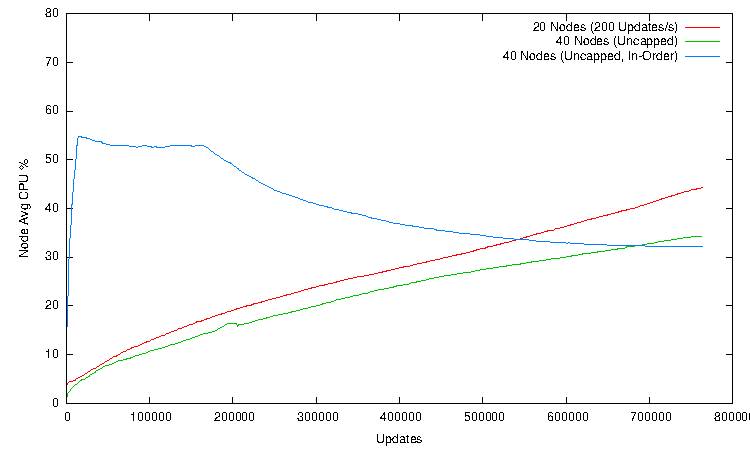
\includegraphics[width=3.0in]{images/100mbUpdatesVsCPUCompletion.pdf} & 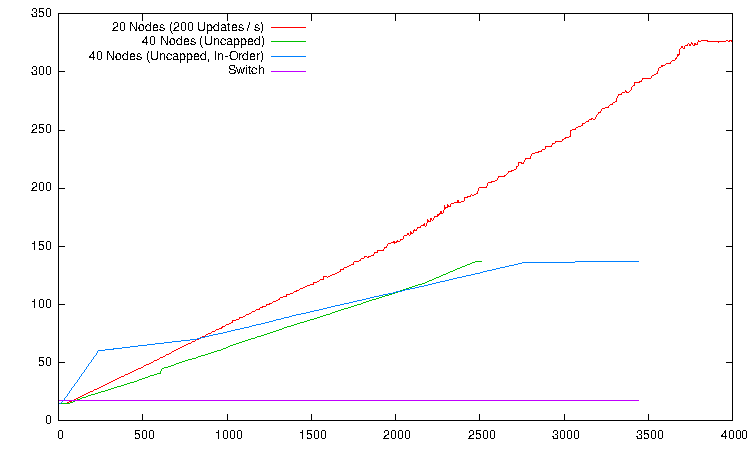
\includegraphics[width=3.0in]{images/100mbUpdatesVsMemory.pdf}\\
(a) & (b) \\
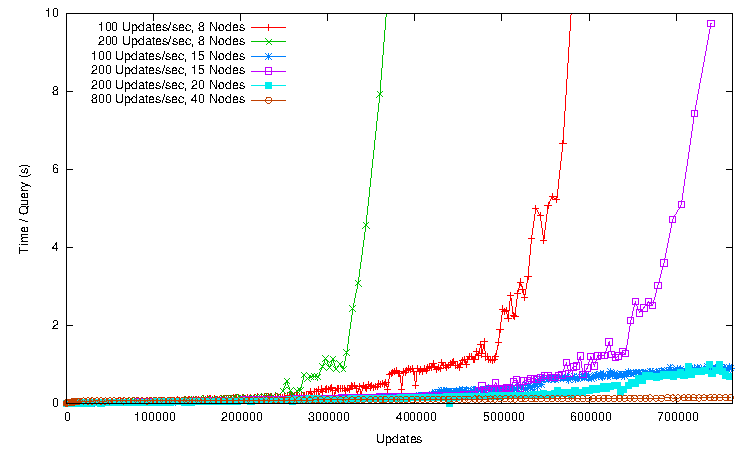
\includegraphics[width=3.0in]{images/expandingbreakdown.pdf} & 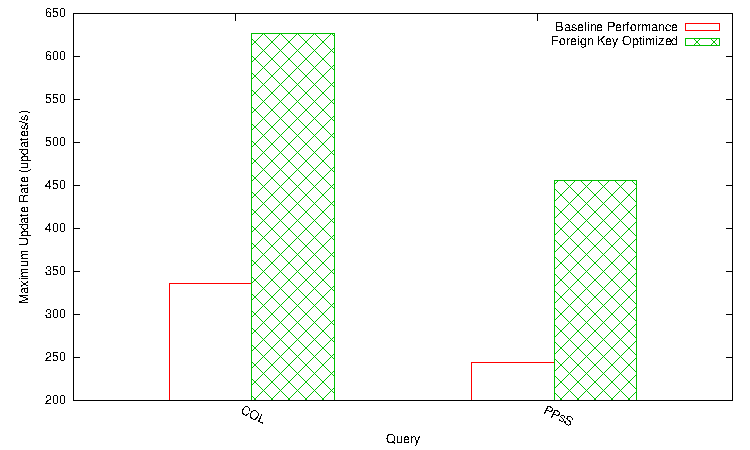
\includegraphics[width=3.0in]{images/foreignkey.pdf}\\
(c) & (d) \\
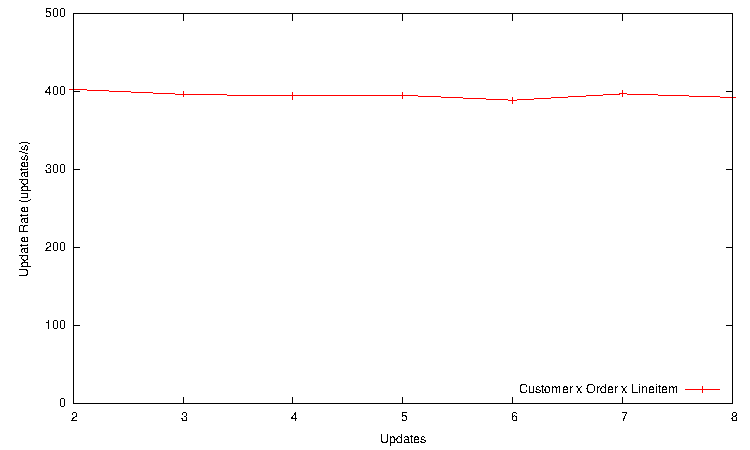
\includegraphics[width=3.0in]{images/aggvsupdates.pdf} & 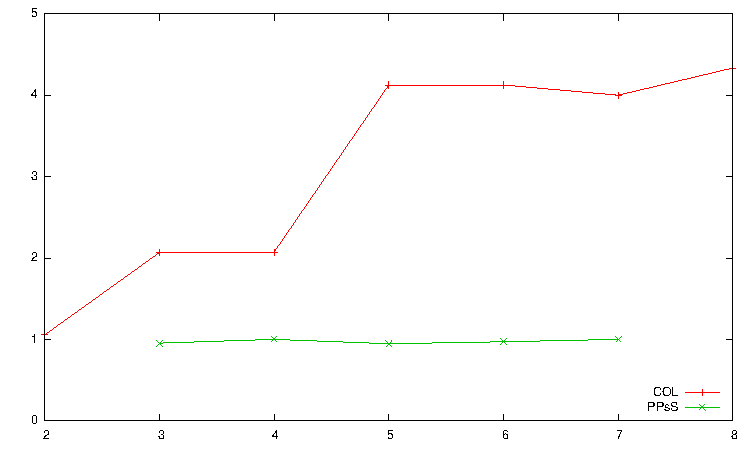
\includegraphics[width=3.0in]{images/aggvslatency.pdf}\\
(e) & (f) \\
\end{tabular}
\caption{(a) CPU Utilization over the course of a series of updates on an empty database.  (b) Memory usage over the course of a series of updates on an empty database.  (c) Query latencies leading up to the node processing breakdown point.  (d) Improvement in update rate as due to the Foreign-Key Join optimization.  (e) Update rate as a function of number of dependent group-by columns added.  (f) Query latency as a function of the number of dependent group-by columns added. }
\label{fig:expandingbreakdown}
\label{fig:20nodes100mbUpdatesVsCPUCompletion}
\label{fig:20nodes100mbUpdatesVsMemory}
\label{fig:fkupdatethroughput}
\label{fig:aggvsupdates}
\label{fig:aggvslatency}
\end{center}
\end{figure*}

\begin{figure}
\begin{tabular}{|c|c|c|c|c|}
\hline
 & \multicolumn{2}{c|} {\textbf Original} & \multicolumn{2}{c|} {\textbf Optimized} \\
{\textbf Query} & {\textbf Maps} & {\textbf Rules} & {\textbf Maps} & {\textbf Rules} \\ \hline
COL  & 6 & 20 & 3 & 6 \\ \hline
PPsS & 10 & 38 & 4 & 10 \\ \hline
\end{tabular}
\caption{Simplication in Cumulus' execution plan as a result of applying the Key-Foreign Key Join optimization for the example queries.}
\label{fig:fkbenefittable}
\end{figure}

\subsection{Scalability}

The first point of our analysis is to study the behavior of Cumulus under increasing load.  We start with an empty database and issue inserts that cause progressively more complex inserts.  Using the COL query to construct the warehouse, we perform Customer, Order, and Lineitem inserts, interleaved with each other.  As the number of inserts grows, so does the frequency with which Orders correspond to already-inserted Customers (and visa versa).  With the increased frequency of correspondence, additional work needs to be done to insert tuples into maps.  

Figure \ref{fig:expandingbreakdown}c tracks the breakdown points of individual Cumulus nodes at varying loads and cluster sizes.  As inserts occur, aggregation queries are posed to the cluster to measure performance.  Query latency remains relatively constant, only growing significantly once the system is saturated by updates.  The elbow in each graph represents the point at which the cluster has reached its processing capacity.  Note that the cluster's processing capacity scales linearly with the cluster size; a 20 node cluster can trivially handle the demands placed on it when every insert is guaranteed to trigger many map updates.  A 40 node cluster not only handles a much higher update rate, but also remains more responsive to OLAP queries as each node is responsible for aggregating a smaller fraction of the data.

We expand on these results, showing the CPU utilization of the 20-node and 40-node cases in Figure \ref{fig:20nodes100mbUpdatesVsCPUCompletion}a, and Memory utilization in Figure \ref{fig:20nodes100mbUpdatesVsMemory}b.  Even as the domains of a given loop variable increase (the sharp increase in the slope of the completion line), per-node processor usage manages to tail off at about 30\%, increasing to 40\% only towards the very end in the 20 node case.  Similarly, despite increased usage due to inefficient memory management in Ruby, node memory usage scales linearly with the amount of data being stored at the node.


\subsection{Key-Foreign Key Join Optimization}
\label{sec:key_fkey}

We next measure the benefits of applying the Key-Foreign Key join optimization described in Section \ref{sec:key_fkey}.  We apply foreign key constraints as documented in the TPC-H specification: 
\begin{itemize}
\item $Order.CustKey$ references $Customer$
\item $Lineitem.OrderKey$ references $Order$
\item $PartSupp.PartKey$ and $PartSupp.SuppKey$ reference $Part$ and $Supplier$, respectively

\end{itemize}

Figure \ref{fig:fkbenefittable} shows how much the M3 statement and maps can be simplified by applying the optimization, and Figure \ref{fig:fkupdatethroughput}d shows the improvement in update throughput.  .  A relatively simple query like $COUNT(*)$ requires only a small number of maps to begin with.  While the number of maps is only reduced by half, the rules are dramatically simplified, each insert or delete fires only a single trigger.

By comparison, a more complex query like PPsS begins with a much greater number of maps in order to store all terms used in the aggregate.  However, because operations on the outermost maps are guaranteed never to affect the query result, most of the intermediate values for each map and the operations required to maintain them can be discarded.

\subsection{Aggregation}
% Removal order: 
% COL: Order.OrderPriority, LineItem.ShipLate, Customer.NID, LineItem.ShipMode, Order.ShipPriority, LineItem.RecvLate
% PPSS: Type, MFGR

Finally, we consider the behavior of Cumulus with respect to redundancy in the query workload.  Figure \ref{fig:aggvsupdates}e shows the update rate as a function of the number of group-by aggregate columns in the query.  For each query, a randomly selected subset of the non-key group-by aggregate terms are removed.  While each group-by column adds another dimension to one or more maps, foreach loops iterate only over values actually defined in the input maps.  Because the removed columns are functionally dependent on at least one of the two remaining key columns, adding them to the query does not de-aggregate the query result and no aditional work is required.

Similarly, Figure \ref{fig:aggvslatency}f shows the effect of de-aggregation on query latency.  As updates occurred within the cluster, th cluster was continuously asked to provide a running count of the sum with no group-by columns.  Shown in the figure is the average response time with respect to the number of group-by columns in the query itself.  Removing all the non-key group-by columns produces a query that groups line-items together.  The factor of four decrease in query processing time corresponds to the average number of lineitems per order.  Combined with Cumulus' processing scalability, this graph demonstrates the feasibility of implementing and incrementally maintaining an entire data-cube in the cloud; The extra work of processing partial aggregates (as in a partially materialized datacube) can be spread out across nodeds in the cloud.  Conversely, an OLAP user need only interact with map partitions for the aggregate closest to their query, limiting the number of message required to pose the query.

